\paragraph{}
Face landmark detection is the process of finding regions (points) of interest (ROI) in an image of a human face, those landmarks are used after wards as input features for our model.
\begin{figure}[H]
	\centering
	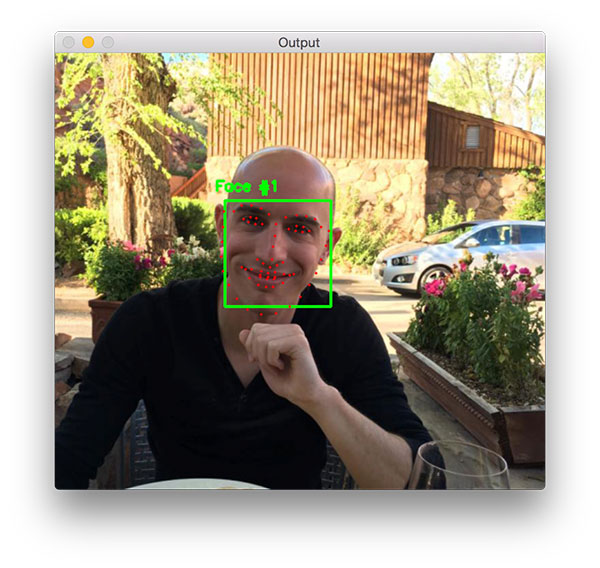
\includegraphics[width=.5\linewidth]{images/lm1.jpg}
	\caption{Landmarks Example}
\end{figure}
\paragraph{}
\textbf{How it works:}\newline
We first detect the face, then mark the regions of interest (landmarks) in it, such as Mouth, Right eyebrow, Left eyebrow, Right eye, Left eye, Nose and Jaw.\newline
\textbf{A pre-trained facial landmark detector inside the dlib library can be used to estimate the location of 68 (x, y)-coordinates that map to facial structures on the face} .

\begin{figure}[H]
	\centering
	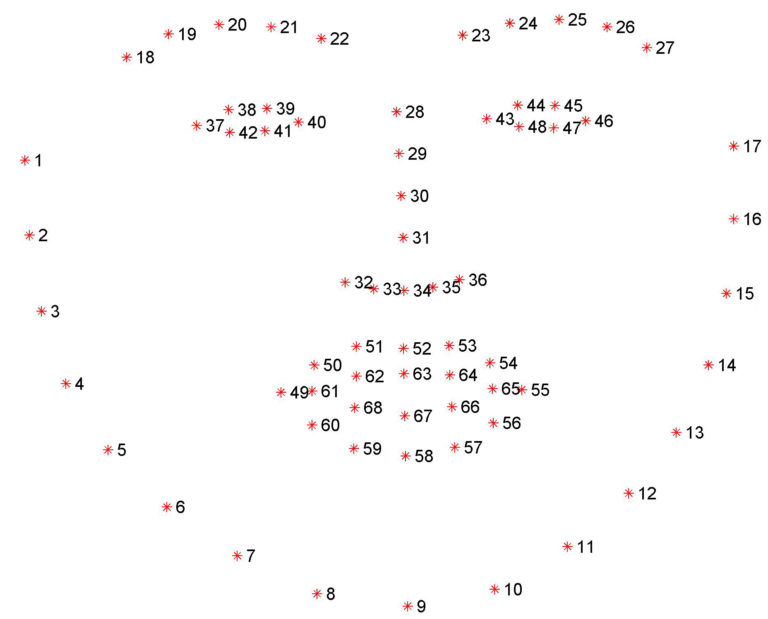
\includegraphics[width=.5\linewidth]{images/lm2.jpg}
	\caption{68 Landmarks Distribution}
\end{figure}

\paragraph{}
The facial landmark detector that we use is included in the dlib library that is an implementation of the One Millisecond Face Alignment with an Ensemble of Regression Trees paper \cite{lm}.\newline
It used a training set of labeled facial landmarks on an image. These images are manually labeled,specifying specific (x, y)-coordinates of regions surrounding each facial structure.\newline
Given this labeled data, an ensemble of regression trees are trained to estimate the facial landmark positions directly from the pixel intensities themselves (i.e., no "feature extraction" is taking place).\newline
The end result is a facial landmark detector that can be used to detect facial landmarks in real-time with high quality predictions.


